\chapter{Implémentation «\texorpdfstring{\,}{\ }classique\texorpdfstring{\,}{\ }»}
    Dans la partie précédente, nous avons discuté de la méthode de Pollard (telle que présentée dans le \textit{Handbook of Applied Cryptography}~\autocite[106]{handbook}) pour résoudre le problème du logarithme discret.

    Un des objectifs de ce projet est de produire un programme capable de résoudre le problème, que l'on peut formaliser de la façon suivante.

    En appelant le programme sur des entiers $p, q, g, h$ respectant~:
    \begin{equation} \label{eq:2}
      \begin{split}
        p \text{\ et } q \text{\ deux nombres premiers} \\
        \text{tels qu'il existe un unique sous-groupe de } {(\mathbb{Z}/p\mathbb{Z})}^* \text{\ d'ordre } q \\
        g \text{\ un générateur de ce groupe multiplicatif, \textit{i.e} } {(\mathbb{Z}/p\mathbb{Z})}^* =\ < g > \\
        h \in {(\mathbb{Z}/p\mathbb{Z})}^*
      \end{split}
    \end{equation}

    Cette dernière condition assure qu'il existe $x \in \mathbb{Z}$ tel que $h = g^x$; ce $x$ correspond à $\log_g(h)$, et c'est ce que l'algorithme retourne.

    Pour des raisons de performances, ce programme est écrit en C.
    Cependant, afin de se familiariser avec la méthode, et nous assister dans la génération de grands nombres $p$, $q$ et d'un générateur $g$ leur correspondant, nous avons commencé par utiliser le logiciel SageMath\footnote{\url{https://www.sagemath.org/}}. De plus, nous avons aussi pu automatiser la génération de données de tests (des entiers $h$ et $x$ respectant $g^x = h$) pour valider le bon fonctionnement du programme, mais aussi mesurer les performances des algorithmes utilisés, afin de pouvoir mettre en perspective d'éventuelles optimisations dont il sera question plus tard.

    Dans ce chapitre, nous allons donc présenter brièvement le premier prototype que nous avons obtenu à l'aide de Sage.
    Bien que non optimisé, cela nous a permis de découvrir quelques questions et contraintes auxquelles nous avons aussi dû répondre lors de l'implémentation en C.
    Nous parlerons de ces problématiques, en particulier de la génération de grands entiers définissant les groupes dans lesquels nous avons travaillé (pour tester et mesurer l'efficacité de notre programme).
    Enfin, nous présenterons le code C ayant permis de générer notre programme de résolution du problème, ainsi que les différents tests et mesures mis en place pour en valider le bon fonctionnement et l'efficacité.


    \section{SageMath}
        \subsection{Prototype de la méthode \texorpdfstring{$\rho$}{Rho}}
        Pour nous aider à prendre en main la méthode, il nous a été proposé de l'implémenter dans un premier temps à l'aide de Sage.

        Nous nous sommes donc appuyés sur les valeurs données dans le Handbook pour tester notre solution.
        Dans les exemples qui vont suivre, nous nous placerons donc dans le sous-groupe de ${(\mathbb{Z}/383\mathbb{Z})}^*$ d'ordre $191$ et dont $2$ est un générateur.

        Dans les grandes lignes, notre programme Sage s'articule autour de trois fonctions~:
        \begin{itemize}
            \item La fonction \lstinline{f} d'itération.
            \item La fonction \lstinline{rho_table}~: appelle la fonction d'itération jusqu'à détecter une collision (en suivant l'algorithme de Floyd\footnote{Présenté en section~\ref{chapter1:Floyd}.}). Notons que cette fonction stocke l'ensemble des valeurs intermédiaires calculées dans un tableau, pour valider visuellement la correspondance entre la table donnée dans le \textit{Handbook}~\autocite[107]{handbook} et les valeurs que l'on obtient.
            \item La fonction de calcul du logarithme discret recherché (sobrement nommée \lstinline{solve}) en fonction des exposants obtenus lors de la collision.
        \end{itemize}

        Notons que ce code est critiquable sur plusieurs points.

        Premièrement, nous n'avons pas cherché à optimiser notre programme, avons mal architecturé les différentes briques logiques, et n'avons porté aucune attention à la gestion mémoire.
        On note donc, parmi les points problématiques de cette implémentation~: mélange des fonctions de calcul et d'affichage et stockage non nécessaire des valeurs intermédiaires (impliquant probablement, dès lors que l'on utilisera de grands nombres, une consommation mémoire démesurée, et des temps de calculs interminables).

        C'est pour contrôler aux mieux ces aspects que nous nous sommes tournés vers le langage C pour implémenter une version efficiente de l'algorithme de Pollard.

        Finalement, obtenir rapidement un prototype de notre solution à l'aide de SageMath nous a permis de soulever ces questions d'organisation du code et d'esquisser l'architecture dont nous aurons besoin lors de l'implémentation en C.
        Mais avant d'entrer dans ces subtils détails, présentons maintenant un autre sujet pour lequel SageMath a été pertinent~: la génération des nombres $p, q, g, h$ respectant les relations définies en \eqref{eq:2}.

        \subsection{Génération de données}
        \label{chapter2:sagemath:data}
        Pour pouvoir tester et comparer nos futures implémentations en C, nous devons générer un ensemble de données.

        Dans un premier temps, nous allons générer des entiers $p, q, g$ représentant le sous-groupe de $\mathbb{Z}/p\mathbb{Z}$ d'ordre $q$ et engendré par $g$, où $p$ et $q$ sont premiers.

        Nous avons choisi de créer un tel groupe grâce à une fonction prenant en paramètres la longueur binaire de $p$ et de $q$.

        Pour ce faire, on choisit tout d'abord $q$ aléatoirement de $k_q$ bits jusqu'à obtenir un entier $q$ qui soit premier (fonction gen\_order).

        Ensuite, on construit $p$ tel que $q$ divise $p - 1$, ce qui assurera le fait qu'il existe un unique sous-groupe de $\mathbb{Z}/p\mathbb{Z}$ d'ordre $q$. Or on a cela si et seulement s'il existe $u \in\mathbb{Z}$ tel que $p = uq + 1$. Si on veut $p$ de $k_p$ bits, on tire $u$ (toujours aléatoirement) de $k_p - k_q$ bits jusqu'à trouver $p = uq + 1$ premier (fonction gen\_modulus).

        On obtient ainsi un sous-groupe $\mathbb{Z}/p\mathbb{Z}$ d'ordre $q$.

        Pour finir, il nous reste à trouver un générateur de ce groupe ainsi formé. On sélectionne un élément $v \in \mathbb{Z}/p\mathbb{Z}$ (concrètement on commence à $v = 2$). On pose alors $g = v^u \text{ mod } p$. Si $g = 1$, on prend un autre élément $v$ (ou on incrémente $v$), sinon $g$ est un générateur du groupe (fonction gen\_group).\\
        En effet, dans ce dernier cas on aura~:
        \begin{align*}
        g^q & = v^{uq} \\
            & = v^{p-1} & \text{ puisque } p = uq + 1 \\
            & = 1 \text{ mod } p & \text{ d'après le petit théorème de Fermat}
        \end{align*}
        Et cela garantit que $g$ est un générateur du sous-groupe de $\mathbb{Z}/p\mathbb{Z}$ d'ordre $q$.\\

        Maintenant que nous avons créé un groupe comme nous le souhaitions, nous allons construire, pour un groupe donné, plusieurs entiers (100 dans notre cas) $h$ et $x$ tels que $g^x = h$ mod $p$. Dans la mesure où nous aurons ce $x$, nous pourrons alors vérifier que nos algorithmes de résolution du problème du logarithme discret rendent bien le résultat attendu.

        Pour cela nous choisissons simplement $x$ aléatoirement, pour ensuite poser $h = g^x$ mod $p$. Notre fonction gen\_data répète ce procédé 100 fois pour ensuite nous retourner ces données.\\

        À présent, grâce à cette dernière fonction, nous pouvons générer un fichier contenant un ensemble de $p, q, g, h, x$ (un par ligne). C'est ce pour quoi nous avons créé la fonction gen\_test\_inputs. Cette fonction construit des groupes d'ordres $q$ de 5 à 55 bits. Pour un $q$ donné de $k_q$ bits, nous prenons un $p$ de $k_q + 10$ bits et avons donc pour chaque couple $(p,q)$ 100 valeurs de $h$ en appliquant la fonction gen\_data.

        Avec ceci, nous pourrons mesurer les performances moyennes de notre programme sur en fonction de la taille de $q$. Dans la prochaine section de ce chapitre, nous parlerons finalement de notre implémentation en C de la résolution du Logarithme Discret, et en présenterons les performances sur le jeu de données que nous venons de générer.

        \section{Implémentation en C}
          Pour l'implémentation de l'algorithme $\rho$ de Pollard en C, nous avons utilisé la bibliothèque GMP\footnote{\url{https://gmplib.org/}}. Cette bibliothèque introduit un nouveau type~: mpz\_t, qui permet de manipuler de grands entiers. Ce type est un peu contraignant à utiliser~: en effet, chaque utilisation d'un mpz\_t doit s'accompagner d'une initialisation (fonction mpz\_init) et d'un "nettoyage" (fonction mpz\_clear). En outre, chaque opération sur des mpz\_t se fait grâce à une fonction prédéfinie~: par exemple, une addition de deux mpz\_t ne se fait pas avec un simple "+", il faut utiliser la fonction mpz\_add. Aussi, nous devons à chaque fois faire une opération après l'autre~: chaque fonction fait une opération entre deux mpz\_t (ou un mpz\_t et un int), mais pas plus.\\

          Par ailleurs, lorsque nous utilisons les mpz\_t, nous avons choisi de passer par des pointeurs afin d'éviter des copies en mémoire inutiles lors de différentes opérations, et cela permet évidemment un gain de temps.\\

          Dans le but de résoudre le problème du logarithme discret, nous avons implémenté plusieurs fonctions, en nous appuyant sur ce que nous avons écrit dans le premier chapitre~:

          \begin{itemize}
            \item La fonction d'itération $f$ (module iteration\_basic.c~\footnote{Disponible \href{https://github.com/Pamplemousse/pollard_rho_algorithm/blob/master/c/iteration_basic.c}{ici}.}) décrite en~\ref{chapter1:iteration_basique}, avec $S_1 = \{ x_i \equiv 1 \text{ mod } 3 \}$, $S_2 = \{ x_i \equiv 0 \text{ mod } 3 \}$ et $S_3 = \{ x_i \equiv 2 \text{ mod } 3 \}$. Étant donnés $x_i$, $a_i$ et $b_i$, elle calcule les termes suivants.
            \item La fonction de détection de cycle de Floyd $collision$ (module collision\_floyd.c~\footnote{Disponible \href{https://github.com/Pamplemousse/pollard_rho_algorithm/blob/master/c/collision_floyd.c}{ici}.}) comme vue en~\ref{chapter1:Floyd}~: à partir d'un couple $(x_i, x_{2i})$, elle calcule grâce à la fonction d'itération $f$, $x_{i+1} = f(x_i)$ et $x_{2(i+1)} = x_{2i+2} = f(f(x_{2i})$, et on s'arrête lorsque l'on trouve $j \in \mathbb{N}$ tel que $x_j = x_{2j} \text{ mod } p$ et $b_j \neq b_{2j} \text{ mod } q$.
            \item La fonction de résolution du problème $discrete\_log\_from\_exponents$ (module equation\_solver.c~\footnote{Disponible \href{https://github.com/Pamplemousse/pollard_rho_algorithm/blob/master/c/equation_solver.c}{ici}.}) utilisant~\eqref{eq:résolution}~: en partant d'un couple obtenu avec la fonction précédente, elle nous rend $\log_g(h)$.
      \end{itemize}


    \section{Tests et mesures}
      Une bonne pratique de développement logiciel consiste à écrire des tests automatisés visant à valider le bon comportement de tout ou partie d'un programme sous certaines conditions et entrées.

      Afin de valider le bon fonctionnement de ce que nous avons produit, nous avons donc mis en place une suite de tests
      \begin{enumerate*}
        \item unitaires \footnote{Visant à valider le fonctionnement des différents modules du logiciel, en vérifiant par exemple le résultat de fonctions sur des entrées spécifiques.}
        \item d'intégration\footnote{Validant le fonctionnement de l'ensemble du programme ; en vérifiant en particulier des résolutions de logarithme discret sur des entiers produits par exponentiation (dont nous connaissons donc le résultat).}
      \end{enumerate*}
      que nous avons écrits.

      Lorsque l'on écrit des tests, il est intéressant d'avoir à l'esprit qu'ils devraient respecter certaines propriétés, connues sous l'acronyme FIRST :
      \begin{itemize}
        \item Fast : les tests s'exécutent rapidement (et il est donc agréable de les lancer régulièrement).
        \item Isolated ou Independent : les tests ne sont pas reliés entre eux, ne contiennent pas d'effets de bords affectant les autres. Nécessaire pour tester de petite unités de notre programme de façon isolée.
        \item Repeatable : les tests produisent toujours le même résultat étant donnée une même entrée. Cela permet de favoriser l'automatisation des tests et d'avoir confiance en ce qui a été testé auparavant.
        \item Self-validating : les tests détectent quand ils passent ou ratent ; il n'est pas nécessaire de forcer un pauvre programmeur à lire des tonnes de logs pour en connaître le résultat.
        \item Timely : les tests sont écrits au même moment que le code qu'ils valident.
      \end{itemize}

      Nous avons donc, au cours du projet, écrit nos propres tests en C (se compilant et s'exécutant comme des programmes à part entière), intégré les tests qui ont jalonné nos avancées, et finalement automatisé des tests plus exotiques \footnote{Écrits en Bash, nous permettant de manipuler facilement les entrées et sorties standard lors de l'appel à l'exécutable produit.}, que nous placerons sous le label "Tests d'intégration" faute de mieux.

      Ces "Tests d'intégration" nous permettent d'assurer la non régression de notre logiciel lorsque nous en changeons le code. En effet, si les tests passent, c'est que le logiciel calcule correctement le logarithme discret sur les entrées pré calculées. Si on modifie notre code (pour introduire une optimisation ou utiliser un autre algorithme), il nous suffit de lancer les tests pour garantir que notre nouveau programme fonctionne (au moins) aussi bien que le précédent.

      Enfin, comme nous souhaitions mesurer et comparer l'efficacité des algorithmes que nous avons implémenté, nous discuterons du "protocole" que nous avons mis en place pour recueillir et traiter les données relatives aux performances de notre programme.


      \subsection{Tests unitaires}
      Comme nous venons brièvement de le présenter, une grande partie de nos tests a consisté en l'écriture de tests "unitaires", validant le fonctionnement de fonctions uniques, sous certaines conditions et paramètres d'entrée spécifiques.
      Sous forme de programme C, chaque jeu de test est contenu dans un fichier et charge le module qu'il est sensé valider. Ensuite, grâce à quelques macros, nous validons le comportement des fonctions dudit module sous différents paramètres.
      Ainsi, et grâce au découpage modulaire de notre programme, nous pouvons attester du bon fonctionnement individuel des différentes fonctions nécessaires à la résolution du logarithme discret.

      Par exemple, ce test permet de valider que la fonction \lstinline{f} retourne un code d'erreur (-1) si le premier paramètre est un pointeur nul~:

      \lstinputlisting[language=C,firstline=32,lastline=36]{code/test_iteration_basic.c}


      \subsection{Tests d'intégration}
      Malheureusement, valider individuellement le comportement de nos fonctions sur certaines entrées ne garantit pas que lorsqu'elles seront utilisées ensemble, le programme se comportera comme nous le souhaiterions.
      Pour se protéger des bugs qui peuvent alors subvenir, nous avons choisi d'écrire des tests de plus "haut niveau", qui valident les sorties du programme sur des entrées contrôlées.

      Clairement, l'idée est la même que pour les tests unitaires : il s'agit de vérifier le comportement du logiciel (au lieu d'un module) sur des entrées prédéfinies. Comme nous interagissons avec notre programme à travers l'interface en ligne de commande (comme vu en section \ref{}), nous avons choisi d'utiliser un outil nous permettant d'écrire des tests en Bash : bash\_unit \footnote{\url{https://github.com/pgrange/bash_unit}}.

      \begin{sloppypar}
        Le code de ces tests est disponible à l'adresse : \url{https://github.com/Pamplemousse/pollard_rho_algorithm/blob/master/c/test/test_pollard_program.sh}.
      \end{sloppypar}

      Ce test s'appuie sur les données générées par la fonction \lstinline{gen_data}, présentée dans la section~\ref{chapter2:sagemath:data}. Pour rappel, ces données consistent en un ensemble de lignes, chacune formatée comme suit : "$p$ $q$ $g$ $h$ $x$", et respectant $h = g^x$ mod $p$.

      Pour chacune de ces lignes, on formate une entrée que notre programme peut reconnaître, puis on l'exécute sur cette entrée, et enfin, on vérifie que le résultat rendu est conforme à ce que l'on sait être la solution du problème sur notre entrée.
<<<<<<< 9a3b987e9ef4981e1b5b085d1e04c680693d43f8
      Ayant généré beaucoup (plus de 200) de ces solutions, en se plaçant sur différents groupes (en faisant varier $p$ et $q$), nous sommes confiant de la santé de notre programme lorsque ces tests passent~: il est capable de calculer correctement des logarithmes discrets.
=======
      Ayant généré beaucoup (plus de 200) de ces solutions, en se plaçant sur différents groupes (en faisant varier $p$ et $q$), nous sommes confiant de la santé de notre programme lorsque ces tests passent : il est capable de calculer correctement des logarithmes discrets.
>>>>>>> [Rapport] Chapitre 2 : Implémentation en C


      \subsection{Mesure de l'efficacité des algorithmes}
      L'intérêt d'implémenter différents algorithmes d'itération et de détection de collision est de pouvoir comparer leurs performances lors du calcul de logarithmes discrets. Nous ne parlerons pas ici de performance en terme de temps (rapidité d'exécution), ni en terme d'espace (quantité de mémoire utilisée), mais nous cherchons plutôt à évaluer le nombre d'appels à la fonction d'itération (on parlera de nombre de cycles) nécessaires en moyenne avant d'obtenir une collision nous permettant de résoudre le problème.

      À partir d'un jeu de données généré comme expliqué dans la section~\ref{chapter2:sagemath:data}, nous avons exécuté notre programme sur différentes entrées, tout en mesurant, lors de chaque résolution, le nombre d'appels à la fonction \lstinline{f} (fonction d'itération) qu'il a été nécessaire d'effectuer avant l'obtention d'une collision.

      Pour nous permettre de mesurer le nombre d'appels à une fonction spécifique dans notre programme, nous avons utilisé GPROF\footnote{\url{https://sourceware.org/binutils/docs/gprof/}}, en compilant notre programme avec les options \lstinline{-pg -no-pie}. Ces options rajoutent des instructions dites "d'instrumentation", qui permettent de collecter des données lors de l'exécution du programme.
      Ainsi, lorsque l'on lance le programme sur une entrée spécifique, un fichier \lstinline{gmon.out} est généré contenant les données de profilage relative à l'exécution qui vient de se passer. Alors, il nous suffit d'utiliser l'utilitaire \lstinline{gprof} pour en extraire ce qui nous intéresse : le nombre d'appels à la fonction d'itération \lstinline{f}, avec la commande suivante~:

      \begin{lstlisting}
        gprof ../c/pollard -b --exec-counts=f
      \end{lstlisting}

      La figure~\ref{fig:generate_measurement_data} nous montre comment nous avons utilisé ce procédé pour prendre des mesures de façon automatique sur le jeu de données que nous avons généré dans la section~\ref{chapter2:sagemath:data}\footnote{Pour rappel, nous avons généré 51 valeurs de $q$ (de taille variant de 5 à 55 bits), pour lesquelles nous avons trouvé un générateur, puis calculé 100 entrées pour le problème du logarithme discret (par exponentiation à une puissance aléatoire). Au total, notre fichier de test contient donc 5100 lignes contenant les entrées et la solution d'un problème de logarithme discret.}.

      \begin{figure}
        \center{}
        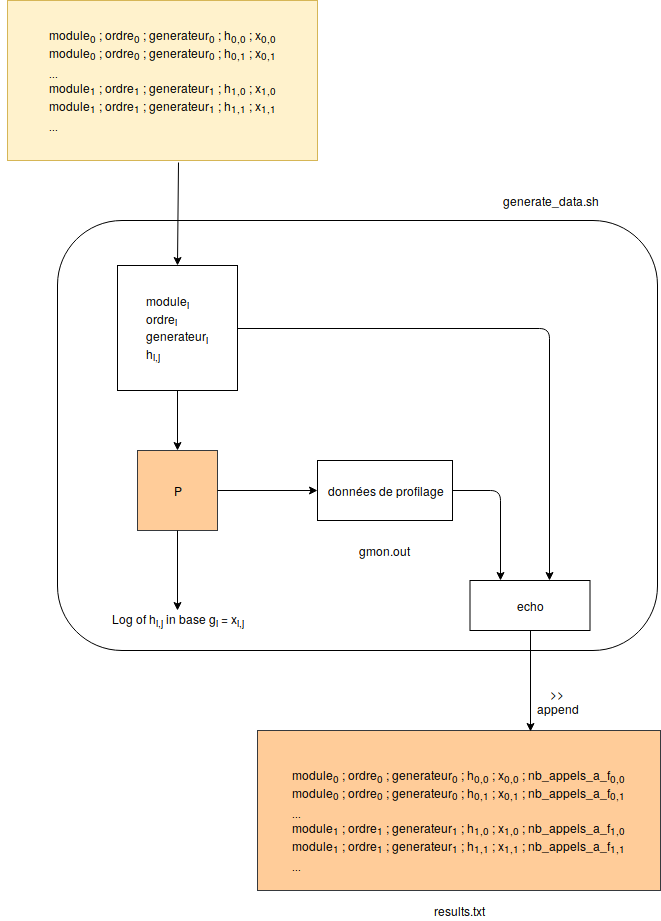
\includegraphics[scale=0.3]{images/generate_measurement_data.png}
        \caption{Agrégation des données générées et des données de profilage}
        \label{fig:generate_measurement_data}
      \end{figure}

      La magie opère à travers le script \lstinline{generate_data.sh}\footnote{Disponible à l'adresse~: \url{https://github.com/Pamplemousse/pollard_rho_algorithm/blob/master/graph/generate_data.sh}}.
      Pour chaque ligne de notre fichier de données, on formate une entrée pour le programme \lstinline{pollard}, dont on profile l'exécution.
      Alors, on récupère le nombre d'appels à la fonction d'itération comme nous venons de le voir, et on ajoute une ligne à notre fichier de sortie suivant le format~: données d'entrées auxquelles on rajoute le nombre que nous venons d'extraire.

      Finalement, nous pouvons traiter les données ainsi recueillies à l'aide de Python et de la librairie Plotly\footnote{\url{https://plot.ly/}} afin d'afficher les résultats obtenus sous forme de graphe.

      Le graphe~\ref{fig:basic_iteration_results} montre les résultats obtenus par notre programme implémentant la méthode de Pollard "originelle", telle que nous l'avons présentée au cours de ce chapitre : utilisant la fonction d'itération présentée dans le \textit{Handbook}~\autocite[107]{handbook} et la méthode du lièvre et de la tortue pour la détection de collisions.

      On peut voir sur ce graphe que la complexité calculatoire de l'algorithme est en $\mathcal{O}(\sqrt{q})$, ce qui confirme les résultats présentés dans le papier originel : \textit{Monte Carlo Methods for Index Computation}\autocite{pollard0}.

      \begin{figure}
        \center{}
        \includegraphics[scale=0.5]{images/iteration_de_base.png}
        \caption{Nombre d'appels à la fonction d'itération avant la détection d'une collision en fonction de la taille de $q$ (l'ordre du groupe)}
        \label{fig:basic_iteration_results}
      \end{figure}


    \paragraph{}
    A présent que nous avons présenté le travail effectué relatif à la méthode de Pollard telle que présentée dans le \textit{Handbook}~\autocite[106]{handbook}, ainsi que les tests et mesures mis en place pour assurer sinon la qualité, au moins le bon fonctionnement de notre implémentation, nous allons dans le prochain chapitre discuter des améliorations possibles à travers de nouveaux algorithmes pour la fonction d'itération, la détection de collision ou la combinaison des deux.
